%-----------------------------------------------------
%  Introduction
%-----------------------------------------------------

\section{서론}

페로브스카이트는 태양 전지에서 빛을 흡수해서 움직이는 전하를 만드는 역할을 한다. 태양 전지가 1970년대 재생 가능 에너지의 일부로써 주목을 받은 이후 지속적인 투자를 받아왔으며 2030년이 되기 전에 광전지로 만드는 전기의 양이 전체 전력의 3분의 1이나 될 것이라는 예측도 있다 \cite{turner2013global}. 
\begin{figure}[h!]
	\begin{center}
		\begin{tabular}{cc}
			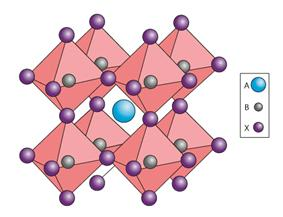
\includegraphics[width=7cm]{perovskite_structure} 
		\end{tabular}
		\caption{The structure of standard perovskite\cite{turner2013global},The octahedral structure on the corner can be seen, made with X. }	
		\label{fig:FIR22}
	\end{center}
\end{figure}
페로브스카이트 재료(이 논문에서 페로브스카이트라고 한다)는 $\rm{ABX_3}$의 결정 구조를 가진 물질로, 여기서 $\rm{A}$, $\rm{B}$는 양이온, X는 음이온이다. 쇼클리-퀴서 한계(Shockley-Quiesser limit) 이론에 의하면, 하나의 p-n 접합에서 1.34eV의 전위차가 걸릴 떄 가장 큰 효율인 33.7 \%가 발생한다고 한다 \cite{ruhle2016tabulated}. 여기서 페로브스카이트의 장점이 대두되는데, A, B, X의 각 구성요소는 상당히 자유롭게 교체할 수 있기 때문에 밴드 간극이 넓은 다양한 페로브스카이트가 만들어질 수 있다. 즉, 전위차를 잘 조절하면 최대 효율을 도달하는 페로브스카이트를 만들 수 있다는 의미이다. 또한, 페로브스카이트는 꼭짓점을 공유하는 팔면체 구조를 가지고 있기 때문에 전하 유동성이 뛰어나다\cite{linaburg2015studies}. 이 특성은 페로브스카이트가 빛을 잘 흡수하고 긴 양공 확산 길이를 가질 수 있게 한다\citen{green2014emergence}. 마지막으로, 페로브스카이트 태양전지는 전통적인 실리콘 태양전지에 비해 쉽게 만들어진다. 페로브스카이트 재료는 100°C 이하로 합성할 수 있는 반면 실리콘 태양전지는 불순물을 제거하기 위해 900°C 이상의 온도가 필요하다.
많은 연구자들과 과학자들은 이러한 장점을 가진 페로브스카이트의 제작 비용, 시간을 줄이고 에너지 전환 효율성을 높이기 위해 활발히 연구하고 있다. 처음으로 페로브 스카이트를 이용하여 빛을 이용한 발전을 한 사람은 Miyasaka였다. 그는 2006년에 처음으로 $\rm{CH_3NH_3PbBr_3}$를 이용한 전지로 2.2%의 효율을 가지는 전지를 만들어 내었다\cite{kojima2006novel}. 2009년에는 Br을 I로 치환하여 효율을 3.8%까지 올렸다\cite{kojima2009organometal}. 연구는 계속되어 2012년 중반에 Snaith가  CH3NH3PbI3−xClx와 같이 17족 원소들을 섞어서 만드는 페로브스카이트가 안정성과 전하 수송 면에서 우수하다는 것을 보였다\cite{lee2012efficient}. Seok(석상일 교수님. 그냥 seok이라고 써도 되는 건가요)은 poly-triarylamine을 CH3NH3PbI3−xBrx와 함께 이용하여 12.3%의 효율을 만들었다\cite{noh2013chemical}. 
최근에는 PDMS(폴리디메틸실록산)를 이용해 단결정 할라이드(hallide) 페로브스카이트를 만드는 새로운 방법이 발견되었다. PDMS는 용액이 웨이퍼에 코팅된 후 압력으로 이을 누르는 데 사용된다. PDMS 스탬핑 없이 AFM(Atomic force microscopy)으로 측정한 거칠기는 79.1 ± 43.3nm이었지만 PDMS 스탬핑은 거칠기를 7.1 ± 4.6nm 로 감소시켰다\cite{khoram2016growth}. 또한, 이 방법은 용액에서 석출하는 방법(Czochralski 방법) 같은 기존의 방법보다 많은 시간을 절약했다. PDMS 스탬프를 적용한 연구에서, 할로겐화 페로브스카이트 필름에 약 130nm 크기의 패턴을 성공적으로 인쇄했다\cite{brittman2017controlling}. 이러한 패턴은 1차원 및 2차원 분산 피드백(DFB) 구조에서 표면 반사율을 감소시켜 효율성을 향상시키기 위해 사용될 수 있다. 
앞선 논문들에서는 PDMS 스탬핑 방식으로 페로브스카이트를 만들긴 했지만 이에 대한 의문을 제기하진 않았다. 새롭게 발견된 방법으로 만들어진 페로브스카이트가 기존의 방법으로 만들어진 페로브스카이트와 같은 특성을 가지고 있다는 것을 증명해야 한다. 이 논문에서는 이를 증명하기 위해 XRD 무늬와 TRPL 분석을 이용하였다. 
XRD(X-Ray Diffraction)은 결정성 물질에 X선을 쏘아 나타나는 고유 무늬로 물질을 구분하는 것이다. 측정기의 각도를 바꿔가며 도달하는 X선의 세기를 측정하여 무늬를 알아낸다. 
TRPL(Time-Resolved Photoluminescence)은 전하 운반자의 시간에 따른 변화를 관찰할 수 있는 장치이다. PL(Photoluminescence)은 물질에 에너지를 가해서 들뜬 상태를 만든 후 물질에서 방출되는 빛을 파장별로 검출하는 방식이다. TRPL은 PL spectra의 시간에 따른 변화를 확인하는 방식으로, 광발광 수명(photoluminescent lifetime)으로 물질을 식별하거나 LED의 효율을 측정되는 데에 쓰인다. 물질마다 TRPL 데이터의 모양이 다른데, 이는 광발광 수명이 물질의 특성이기 때문이다. CsPbBr3의 경우에는 PL의 시간에 따른 변화가 exciton과 biexciton의 재결합에 의해 일어나는데, 각각의 수명은 1170±10ps와 510±5ps이다\cite{chen2018room}. 
이렇게 본 논문은 XRD와 TRPL 분석 방법을 이용하여 PDMS 스탬핑을 이용한 새로운 방법이 페로브스카이트를 합성할 수 있다는 것을 제시한다. 

